\documentclass[conference]{IEEEtran}
\IEEEoverridecommandlockouts
% The preceding line is only needed to identify funding in the
%first footnote. If that is unneeded, please comment it out.
\usepackage{cite}
\usepackage{amsmath,amssymb,amsfonts}
\usepackage{algorithmic}
\usepackage{graphicx}
\usepackage{textcomp}
\usepackage{xcolor}
 \usepackage{multirow}
\def\BibTeX{{\rm B\kern-.05em{\sc i\kern-.025em b}\kern-.08em
    T\kern-.1667em\lower.7ex\hbox{E}\kern-.125emX}}


\usepackage{graphicx}
  % declare the path(s) where your graphic files are
  % \graphicspath{{../pdf/}{../jpeg/}}
% and their extensions so you won't have to specify these with
%  % every instance of \includegraphics




\begin{document}



\title{Security Assessment of Libyan Government Websites}

\author{\IEEEauthorblockN{Abdullah Ahmed Ali, Mohd Zamri Murah}
\IEEEauthorblockA{\textit{Center for CyberSecurity} \\
\textit{Universiti Kebangsaan Malaysia}\\
Malaysia\\
email: abdullah.alhanash@gmail.com\\
zamri@ukm.edu.my}
}

\maketitle

\begin{abstract}
Many governments organizations in Libya have started
transferring traditional government services to
e-government. These e-services will
benefit a wide range of public. However, deployment of
e-government
bring many new security issues. Attackers would take advantages
of vulnerabilities in these e-services and would conduct cyber
attacks that would result in data loss, services interruptions, privacy loss,
financial loss, and other significant loss. The
number of vulnerabilities in e-services have increase due to the complexity of the e-services system, a
lack of secure programming practices, miss-configuration of
systems and web applications vulnerabilities, or not staying up-to-date with
security patches. Unfortunately, there is a lack of study being done to assess the current security level of Libyan government websites. Therefore, this study aims to assess the current security of 16 Libyan government websites using penetration testing framework.
In this assessment, no exploits were committed or tried on the websites. In penetration testing framework (pen test), there are four main phases: Reconnaissance, Scanning, Enumeration, Vulnerability
Assessment and, SSL encryption evaluation. The aim of a security assessment is to discover vulnerabilities that could be exploited by attackers.
We also conducted a
Content Analysis phase for all websites. In this phase,
we searched for security and privacy policies implementation information on
the government websites. The aim is to determine whether the websites are aware of current accepted standard for security and privacy.
From our security assessment results of 16 Libyan government websites, we compared the websites based on the number of
vulnerabilities found and the level of security policies. We only found 9 websites with high and medium vulnerabilities. Many of these vulnerabilities are due to outdated software and systems, miss-configuration of systems and not applying the latest security patches. These vulnerabilities could be used by cyber hackers to attack the systems and caused damages to the systems. Also, we found 5 websites didn't implement any SSL encryption for data transactions.
Lastly, only 2 websites have published security and privacy policies on their websites. This seems to indicate that these websites were not concerned with current standard in security and privacy. Finally, we classify the 16 websites into 4 safety categories: highly unsafe, unsafe, somewhat unsafe and safe. We found only 1 website with a highly unsafe ranking. Based on our finding, we concluded that the security level of the Libyan government websites are adequate, but can be further improved. However, immediate actions need to be taken to mitigate possible cyber attacks by fixing the vulnerabilities and implementing SSL encryption. Also, the websites need to publish their security and privacy policy so the users could trust their websites.


\end{abstract}

\begin{IEEEkeywords}
Libya E-government, Security Assessment, Information Security,
Website Vulnerability, Penetration Testing
\end{IEEEkeywords}

\section{Introduction}

Internet technology has made a massive contribution to communication
and information sharing. There is no doubt that the Internet has made
people’s lives easier and more convenient. Due to this, many
institutions and organizations (both private and government
sectors) see the ease in information sharing and offering online
services, as an opportunity to improve efficiency, transparency,
competitiveness and to survive in the global economy\cite{othman2018whole}\cite{yusof2013evaluating}. 
Many organizations
transferred traditional services into e-services. People can access such
e-services online from any location, any time and cost-effective.

However, the rise of
transferring into e-services brought a new security threat that could affect
confidentiality, integrity and availability of 
information or even threat on the national security of a country. Sharing
information by the private sectors could cause threats to a company, but for the
government sectors, it could be more catastrophic. Therefore,
government sectors need to be more concerned about sharing
information and implementing e-services\cite{zhao2010opportunities}
\cite{kasimin2013using}.

There are many recent cyber attacks toward governments
websites\cite{zhao2010opportunities}. These attacks exploited various
vulnerabilities in the operating systems, network protocol, data
encryption, and web applications. As a result, many governments agencies suffered huge losses
in term of sensitive data, loss of faith among the users and financial losses\cite{tehrani2013cyber}.
Therefore, there is an urgent need to assess and to evaluate existing government
websites as a method to alleviate potential losses from cyber
attacks\cite{al2015security}.

Libyan government websites are also susceptible to cyber
attacks\cite{ihmouda2013penetration}. Current, the is no effort
to assess the security level of the websites. This is probably
due to lack of security experts in Libya, or lack of security
awareness among the government agencies. This situation is not
good for Internet security\cite{yusof2011cyber}.

Due to a lack of security assessment toward Libya government
agencies in current literature, in this paper we took the
initiative to conduct a passive penetration testing on Libya
government websites. We followed a standard penetration testing
framework for
websites\cite{srinivasan2017web,antunes2014penetration}, and
also, assess the security policy of each website.

\section{Methodology}

Our security assessment methodology is based on  
a standard penetration testing guideline\cite{weidman2014penetration}\cite{felderer2016security}.
The assessment and data collection were done
in May 2018. The assessment was based on 16 Libyan
government
websites covering the domain \emph{gov.ly}. The assessment consists of
four
stages as shown in Figure~\ref{fig:steps}.


\begin{figure}[htbp]
\centerline{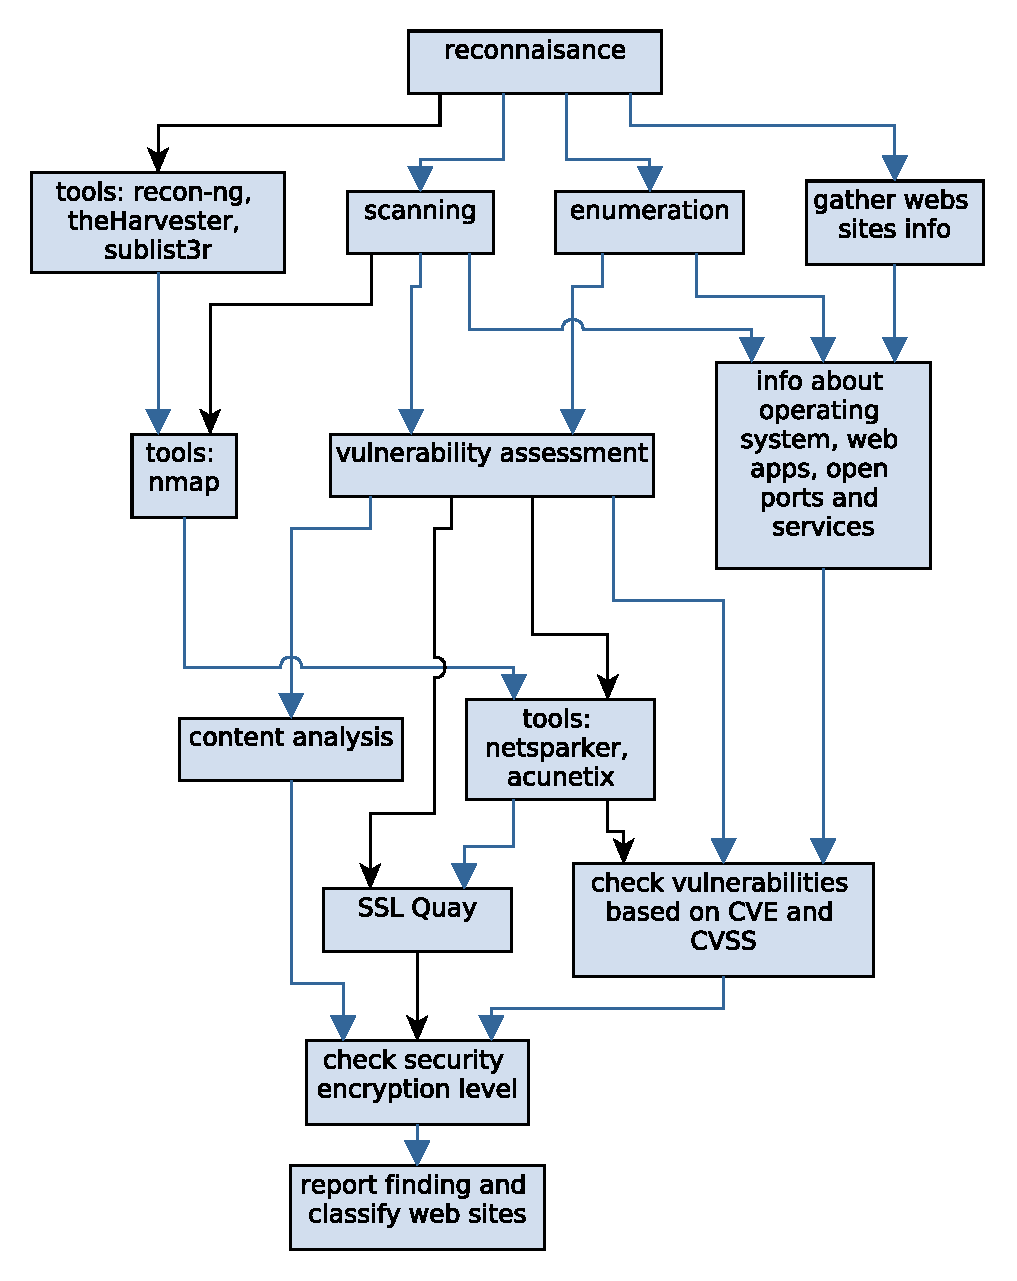
\includegraphics[width=2.5in]{steps.pdf}}
% where an .eps filename suffix will be assumed under latex, 
% and a .pdf suffix will be assumed for pdflatex; 
% or what has been declared
% via \DeclareGraphicsExtensions.
\caption{The security assessment phases. This assessment
consists of
 four major phases; reconnaissance, enumeration and scanning,
  vulnerability assessment, content analysis.}
\label{fig:steps}
\end{figure}


%\begin{table}[htbp]
%\caption{Table Type Styles}
%\begin{center}
%\begin{tabular}{|c|c|c|c|}
%\hline
%\textbf{Table}&\multicolumn{3}{|c|}{\textbf{Table Column Head}}\\
%\cline{2-4} 
%\textbf{Head} & \textbf{\textit{Table column subhead}}&
%\textbf{\textit{Subhead}}& \textbf{\textit{Subhead}} \\
%\hline
%copy& More table copy$^{\mathrm{a}}$& &  \\
%\hline
%\multicolumn{4}{l}{$^{\mathrm{a}}$Sample of a Table footnote.}
%\end{tabular}
%\label{tab1}
%\end{center}
%\end{table}
%
%\begin{figure}[htbp]
%\centerline{\includegraphics{fig1.png}}
%\caption{Example of a figure caption.}
%\label{fig}
%\end{figure}

The first phase (Reconnaissance) is about searching for Libyan
government websites under the domain \emph{gov.ly}. We used an open source tool 
\emph{theHarvester} 
to search for subdomains of \emph{gov.ly}. The result obtained from
\emph{theHarvester} tool was about 742 subdomains. Based on
our analysis, the main domains from 742 \emph{gov.ly} subdomains
were 37 Libyan government websites. After that, we verified these
government websites one after the other manually by accessing their main
pages. We verified if they were active and whether they were related to the current official
government or not. We found that only 16 of the 37 Libyan government
websites were active and related to the current Libyan government.

The second phase (Enumeration and Scanning) is about searching for sensitive information about the websites from the 16 Libyan government websites using \emph{nmap}. This is to determine the security level of the websites. We tried to detect important information such as
operating systems type, open ports, services and main IPs. 

The third phase (Vulnerability Assessment) consists of two types of
vulnerability assessment: web vulnerability scanning and secure socket layer (SSL) encryption evaluating. 
In web vulnerability scanning, we used two web security scanners namely: \emph{Acunetix}
and \emph{Netsparker} to scan for web application vulnerabilities in
the 16 websites. The scanners reported the vulnerabilities and
classified them based on Common Vulnerabilities and Exposures (CVE)
categories as: Critical, high, Medium, low and informational.

The second type of vulnerability assessment is evaluating SSL
encryption of the 16 websites using Qualys SSL Labs rating. This evaluation classifies the websites into different rating: A,B,T, and No
SSL. The rating depends on some factors such as: certificate validation,
different protocols support, key exchange strength and cipher strength.

The fourth phase (Content Analysis) searches the websites for their published security and 
privacy policies. The search
includes checking whether the policies are published in the main pages
with clear links or not. The search was carried out manually
by accessing each of the 16 websites and try to find the links for security and privacy policies. The fourth phase is not in any current security assessment framework, but our extra assessment for the websites.

\section{Result and Analysis} \label{sec:result}

%The result is divides into two main phases:
%\begin{enumerate}
%\item showing the results of security assessment
%phases: Reconnaissance, Enumeration and Scanning, Vulnerability Assessment, and
%Content Analysis.
%\item analyzing the vulnerabilities and classifying
%websites security.
%\end{enumerate}

\subsection{Reconnaissance phase}

In the Reconnaissance phase, we discovered 742 subdomain in \emph{gov.ly} domain. We pick 16 websites for further analysis.

\subsection{Enumeration and Scanning}

In the scanning phase, we discovered operating system for 11 websites, running services from 16 websites, open ports on all 16 websites and IP numbers from 14 websites. Many of the websites are still using outdated operating system such as Linux 2.0 series and old version of Windows operating system. 

This information is important because it could be used by cyber attackers to attack the systems. Counter measures should be implemented to hide the operating system, closes all unnecessary ports, stop unnecessary services and use web application firewalls to secure the websites. 

%\begin{table}[htbp]
%\caption{After the Reconnaissance phase, we picked 16 government websites. The information we obtain are summarized below.
%For example, we obtain operating system information from 11
%hosts, services
%available from 16 hosts, open ports from 16 hosts, and IP
%number from 14 hosts.}
%\label{tab:nmap}
%\centering
%\begin{tabular}{@{}lllll@{}}
%\hline & \begin{tabular}[c]{@{}l@{}}operating\\
%system\end{tabular}
%  & services & open ports & host IPs \\
%  \hline & 11 & 16 & 16 & 14 \\
%  \hline
%\end{tabular}
%\end{table}

\subsection{Security assessment}

%Results of scanning and enumeration phase showed that \emph{nmap} tool
%detected the
%operating systems for 11 websites, main IP addresses for 14
%websites,
%services and open ports for all 16 websites. This is summarize
%in table~\ref{tab:nmap}. 

The vulnerability assessment phase is divided
into web vulnerability
scanning and SSL encryption evaluation. The web vulnerability scanning used
\emph{Acunetix} and \emph{Netsparker} to identify web application vulnerabilities. The scanning process would took a long time because the web scanner would crawl the websites and look for vulnerabilities one by one. These vulnerabilities are
based on CVE and CVSS\cite{makino2015evaluation,basto2017comparison}, a commonly accepted ranking and description of vulnerabilities.

Based on these two scanners we 
identified 1 critical vulnerability, 24 high vulnerabilities, 139 medium
vulnerabilities, 129 low vulnerabilities and 229 informational
vulnerabilities from 16 websites. It was important to note that results from \emph{Acunetix} and \emph{Netsparker} were different because each of them used different algorithms to find the vulnerabilities.

%This is summarize in table~\ref{tab:vuln}.

We also categorized the 16 websites based on the number of web vulnerabilities found. We have 1 website  with 1 critical vulnerability, 7 websites have high vulnerabilities, 15 websites have medium vulnerabilities, and 15 websites have low vulnerability. 

%\begin{table}[]
%%\centering
%\caption{Overall numbers of vulnerabilities detected from 16
%  websites. The claasification of the vulnerabilities are based on Common
%  Vulnerabilities and Exposures (CVE) and CVSS}
%\label{tab:vuln}
%\centering
%\begin{tabular}{lllll}
%  \hline
%info & low & medium & high & critical \\ \hline
%229  & 129 & 139    & 24   & 1       
%\end{tabular}
%\end{table}



%\begin{table}[]
%%\centering
%  \caption{The numbers of websites with the above mentioned
%vulnerabilities. For example, there are 7 sites that have high
%vulnerabilities.}
%\label{tab:sites}
%\centering
%\begin{tabular}{lllll}
%  \hline
%info & low & medium & high & critical \\ \hline
%16  & 15 & 15    & 7   & 1 \\
%\hline       
%\end{tabular}
%\end{table}

We discovered vulnerabilities both based on the web
applications and the systems deployed. These vulnerabilities are shown in Table~\ref{tab:apps}. The table shows vulnerabilities commonly
found on the 16 websites. The vulnerabilities classified by \emph{Acunetix} and \emph{Netsparker} into
\textbf{Critical}, \textbf{High}, \textbf{Medium}, \textbf{Low} and 
\textbf{Informational} depending on Common
Vulnerabilities and Exposures (CVE) scoring. The CVE is an accepted
standard for publicly disclosed of cyber security vulnerabilities and exposures\cite{makino2015evaluation}.

\renewcommand{\arraystretch}{1.3}

\begin{table}[]
\caption{the vulnerabilities commonly found in the 16
websites and their criticality}
\label{tab:apps}
\centering
\begin{tabular}{lll}
\textbf{vulnerabilities} &
\textbf{\begin{tabular}[c]{@{}l@{}}number
    of\\ occurance\end{tabular}} &
\textbf{\begin{tabular}[c]{@{}l@{}}level of\\ risk\end{tabular}}\\ \hline
WordPress CMS & 5 & high \\ out of date PHP & 2 & high \\
\begin{tabular}[c]{@{}l@{}}Cross-site Scripting\\
(XSS)\end{tabular}& 5 & high \\
\begin{tabular}[c]{@{}l@{}}application error\\
messages\end{tabular}& 78& medium \\
\begin{tabular}[c]{@{}l@{}}Cross-Site Request Forgery\\
(CSRF)\end{tabular} & 4 & medium \\
out of date jQuery & 12 & medium \\
\begin{tabular}[c]{@{}l@{}}PHP information \\
disclosure\end{tabular}& 3 & medium \\
\begin{tabular}[c]{@{}l@{}}PHP code execution\\ and
DOS\end{tabular} & 3 & medium \\
\begin{tabular}[c]{@{}l@{}}User credentials are sent\\ in clear
text\end{tabular} & 2 & medium \\ \hline
\end{tabular}
\end{table}




\subsection{SSL encryption evaluation}

The second type of assessment is SSL encryption evaluation
using \emph{Qualys SSL Labs} tool. This assessment rated the websites into 4 rating: A, B, T, No SSL. From the result, we found 3 websites rated \emph{A}, 7 websites rated \emph{B}, 1 websites rated \emph{T} and 5 websites rated \emph{No SSL}. The websites rated B have weaknesses 
in key exchange 
which may affect
the encryption by allowing cyber attackers to perform
man-in-the-middle
attack (MITM) and gain access to the communication
channel. We discovered that the T rated websites is one of the important websites that many users utilize in sharing private information. The website is rated T is because the expiration of SSL certificate used on the website, which may lead to a MITM attack.

\subsection{Content Analysis}

The Content Analysis phase showed that only 3 of the 16 websites
provided links to security and privacy policies. One website indicated only published security
policy for the whole organization but did not provide security policy for accessing websites. One website
provided links of privacy and security policies, but the links
were not working. The other 13 websites did not publish any privacy or
security policies.

\section{Discussion and Contribution}

Based on our security assessment of 16 Libyan government websites, we conclude that the current security websites of the 16 websites are adequate. There are only 24 high vulnerabilities and 1 critical vulnerabilities among the 16 websites. Also, we found that only 8 websites have critical vulnerabilities and above.

Based on SSL evaluation, we discovered only 3 websites have a proper SSL A-level accreditation while 13 other either have no SSL implementation or low  level SSL-accreditation. This is a serious issue for the government agencies especially for government agencies that involves in financial or personal data transactions.

Based on our security assessment results from
section~\ref{sec:result},
we proposed a new safety classification matrix for the 16
websites using
four safety categories: highly unsafe, unsafe, somewhat unsafe, safe. This classification will combine 3 different results from
vulnerabilities analysis, content analysis
and SSL encryption evaluation. The purpose of this proposed safety classification is to combine web vulnerabilities with SSL encryption evaluation and come up with a new
safety ranking.

The safety classification model was based on \emph{Netsparker} as
a baseline. Our safety classification model is an overall evaluation of the
security assessment based on web vulnerabilities, content analysis and SSL evaluation. 
In this model, a website safety is based on the number and the type of
vulnerabilities found, the level of SSL implementation and 
the security and privacy policies implementation.

To measure a website safely level, we will first analyze each of
the vulnerabilities for a website. Then, we determine
whether a sensitive information is encrypted or not encrypted during data transaction using at that website. Finally, we 
determine the level of SSL encryption used on the website. Based on our
analysis, we would then
determine the safety level based on Table~\ref{tab:class}. As an example, 
%based on Table~\ref{tab:class}, 
we have a website with 
15 vulnerabilities (2 high, 5 medium, 0 low, 8 informational), a B-rated SSL implementation and no security and privacy policy. In this case, we would classify this website as B(unsafe) because the number of high vulnerabilities are low and B-rated SSL implementation. 

\renewcommand{\arraystretch}{1.3}
% Please add the following required packages to your document preamble:
% \usepackage{multirow}
% Please add the following required packages to your document preamble:
% \usepackage{multirow}
\begin{table}[thbp]
\caption{Classification of a website based on security
assessment, SSL encryption evaluation and content analysis. 
In this classification, there are 4 level of safe. These levels are A(highly unsafe), B(unsafe),C(somewhat unsafe) and D(safe).}
\label{tab:class}
\centering
\begin{tabular}{llclll}
 &  & \multicolumn{4}{c}{\textbf{SSL rating}} \\ \cline{3-6} 
\textbf{\begin{tabular}[c]{@{}l@{}}risk\\ category\end{tabular}}& \textbf{\begin{tabular}[c]{@{}l@{}}sensitive\\
info\end{tabular}} & \textbf{A} & \textbf{B} & \textbf{T} &
\textbf{no SSL} \\ \hline
\multirow{2}{*}{\textit{critical}} & unencrypted & A & A & A & A\\
 & encrypted & B & B & A & A \\ \hline
\multirow{2}{*}{\textit{high}} & unencrypted & B & B & B & B \\
& encrypted & C & C & B & B \\ \hline
\multirow{2}{*}{\textit{medium}} & unencrypted & C & C & C & B
\\
 & encrypted & C & C & C & C \\ \hline
\multirow{2}{*}{\textit{low}} & unencrypted & C & C & C & C \\ &
encrypted & D & D & C & C \\ \hline
\multirow{2}{*}{\textit{info}} & unencrypted & D & D & C & C \\
\cline{2-6}
 & encrypted & D & D & D & C \\ \hline
\end{tabular}
\end{table}

\renewcommand{\arraystretch}{1.3}
% Please add the following required packages to your document preamble:
% \usepackage{multirow}
% Please add the following required packages to your document preamble:
% \usepackage{multirow}
%\begin{table}[thbp]
%\caption{An example of calculating safety level of a website.
%Each vulnerabilities
%will be assessed based on the table. The numbers in the table
%indicate the count of vulnerabilities at that level.}
%\label{tab:class}
%\begin{tabular}{llclll}
% &  & \multicolumn{4}{c}{\textbf{SSL rating}} \\ \cline{3-6} 
%\textbf{\begin{tabular}[c]{@{}l@{}}risk\\ category\end{tabular}}& \textbf{\begin{tabular}[c]{@{}l@{}}sensitive\\
%info\end{tabular}} & \textbf{A} & \textbf{B} & \textbf{T} &
%\textbf{no SSL} \\ \hline
%\multirow{2}{*}{\textit{critical}} & unencrypted & - & - & 1 & -\\
% & encrypted & 2 & 2 & - & - \\ \hline
%\multirow{2}{*}{\textit{high}} & unencrypted & 1 & 1 & 2 & 1 \\
%& encrypted & - & - & - & - \\ \hline
%\multirow{2}{*}{\textit{medium}} & unencrypted & 1 & 1 & - & -
%\\
% & encrypted & - & - & - & - \\ \hline
%\multirow{2}{*}{\textit{low}} & unencrypted & - & - & 1 & - \\ &
%encrypted & - & - & - & - \\ \hline
%\multirow{2}{*}{\textit{info}} & unencrypted & - & 1 & 1 & - \\
%\cline{2-6}
% & encrypted & - & - & - & - \\ \hline
%\end{tabular}
%\end{table}



Based on our analysis on the 16 Libyan government websites, we
concluded that;
\begin{enumerate}
	\item 1 website as highly unsafe. This website has 1 critical vulnerability and no SSL implementation.
	\item 6 websites as unsafe. These websites have the number of high vulnerabilities more than 3 and B-rated or A-rated SSL implementation.
	\item 8 websites as somewhat unsafe. These websites have the number of high vulnerabilities less than 3 and B-rated SSL implementation.
	\item 1 website as safe. This website has 0 high and medium vulnerabilities and A-rated SSL implementation.
\end{enumerate} 

 

\section{Conclusion}


In this paper, we conducted a security assessment of 16 Libyan government
websites
under the domain \emph{gov.ly}. This security assessment consists of  four phases: Reconnaissance, Scanning and Enumeration, Vulnerabilities Assessment, and Content Analysis. In the reconnaissance phase, we obtained information about websites and verifying
them. In the enumeration phase, we detected
information about websites environments and network. In the 
vulnerability assessment, we used two types of assessments:
web vulnerability scanning and SSL
encryption evaluation. Also, we conducted a manual
content
analysis to find whether a website has a security and privacy  policy, and whether the policy is published or not.  Finally, we develop a safety evaluation model that combined vulnerabilities assessment, content analysis and SSL evaluation. The safety ranking would provide another info about the website security status.  Based on the results, we highly recommend to the websites with high number of vulnerabilities to keep up to date with the latest security features to mitigate
possible hacking attempts on their websites. They should also publish
security and privacy policies for the websites in order to increase users trust in the websites.


% Generated by IEEEtran.bst, version: 1.14 (2015/08/26)
\begin{thebibliography}{10}
	\providecommand{\url}[1]{#1}
	\csname url@samestyle\endcsname
	\providecommand{\newblock}{\relax}
	\providecommand{\bibinfo}[2]{#2}
	\providecommand{\BIBentrySTDinterwordspacing}{\spaceskip=0pt\relax}
	\providecommand{\BIBentryALTinterwordstretchfactor}{4}
	\providecommand{\BIBentryALTinterwordspacing}{\spaceskip=\fontdimen2\font plus
		\BIBentryALTinterwordstretchfactor\fontdimen3\font minus
		\fontdimen4\font\relax}
	\providecommand{\BIBforeignlanguage}[2]{{%
			\expandafter\ifx\csname l@#1\endcsname\relax
			\typeout{** WARNING: IEEEtran.bst: No hyphenation pattern has been}%
			\typeout{** loaded for the language `#1'. Using the pattern for}%
			\typeout{** the default language instead.}%
			\else
			\language=\csname l@#1\endcsname
			\fi
			#2}}
	\providecommand{\BIBdecl}{\relax}
	\BIBdecl
	
	\bibitem{othman2018whole}
	M.~H. Othman and R.~Razali, ``Whole of government critical success factors
	towards integrated e-government services: A preliminary review,''
	\emph{Jurnal Pengurusan (UKM Journal of Management)}, vol.~53, 2018.
	
	\bibitem{yusof2013evaluating}
	M.~M. Yusof and A.~Y.~A. Yusuff, ``Evaluating e-government system effectiveness
	using an integrated socio-technical and fit approach,'' \emph{Information
		Technology Journal}, vol.~12, no.~5, pp. 894--906, 2013.
	
	\bibitem{zhao2010opportunities}
	J.~J. Zhao and S.~Y. Zhao, ``Opportunities and threats: A security assessment
	of state e-government websites,'' \emph{Government Information Quarterly},
	vol.~27, no.~1, pp. 49--56, 2010.
	
	\bibitem{kasimin2013using}
	H.~Kasimin, A.~Aman, and Z.~M. Noor, ``Using evaluation to support
	organizational learning in e-government system: A case of malaysia
	government,'' \emph{International Journal of Electronic Government Research
		(IJEGR)}, vol.~9, no.~1, pp. 45--64, 2013.
	
	\bibitem{tehrani2013cyber}
	P.~M. Tehrani, N.~A. Manap, and H.~Taji, ``Cyber terrorism challenges: The need
	for a global response to a multi-jurisdictional crime,'' \emph{Computer Law
		\& Security Review}, vol.~29, no.~3, pp. 207--215, 2013.
	
	\bibitem{al2015security}
	M.~S. Al-Sanea and A.~A. Al-Daraiseh, ``Security evaluation of saudi arabia's
	websites using open source tools,'' in \emph{2015 First International
		Conference on Anti-Cybercrime (ICACC)}.\hskip 1em plus 0.5em minus
	0.4em\relax IEEE, 2015, pp. 1--5.
	
	\bibitem{ihmouda2013penetration}
	R.~Ihmouda, N.~H. Alwi~Mohd \emph{et~al.}, ``Penetration testing for libyan
	government website,'' in \emph{International Conference on Computing and
		Informatics}.\hskip 1em plus 0.5em minus 0.4em\relax Universiti Utara
	Malaysia-Uum, 2013.
	
	\bibitem{yusof2011cyber}
	A.~R.~M. Yusof, M.~F. Sukimi, S.~B. Ismail, and Z.~B. Othman, ``The cyber space
	and information, communication and technology: A tool for westernization or
	orientalism or both,'' \emph{Journal of Computer Science}, vol.~7, no.~12,
	pp. 1784--1792, 2011.
	
	\bibitem{srinivasan2017web}
	S.~M. Srinivasan and R.~S. Sangwan, ``Web app security: A comparison and
	categorization of testing frameworks,'' \emph{IEEE Software}, no.~1, pp.
	99--102, 2017.
	
	\bibitem{antunes2014penetration}
	N.~Antunes and M.~Vieira, ``Penetration testing for web services,''
	\emph{Computer}, vol.~47, no.~2, pp. 30--36, 2014.
	
	\bibitem{weidman2014penetration}
	G.~Weidman, \emph{Penetration testing: a hands-on introduction to
		hacking}.\hskip 1em plus 0.5em minus 0.4em\relax No Starch Press, 2014.
	
	\bibitem{felderer2016security}
	M.~Felderer, M.~B{\"u}chler, M.~Johns, A.~D. Brucker, R.~Breu, and
	A.~Pretschner, ``Security testing: A survey,'' in \emph{Advances in
		Computers}.\hskip 1em plus 0.5em minus 0.4em\relax Elsevier, 2016, vol. 101,
	pp. 1--51.
	
	\bibitem{makino2015evaluation}
	Y.~Makino and V.~Klyuev, ``Evaluation of web vulnerability scanners,'' in
	\emph{Intelligent Data Acquisition and Advanced Computing Systems: Technology
		and Applications (IDAACS), 2015 IEEE 8th International Conference on},
	vol.~1.\hskip 1em plus 0.5em minus 0.4em\relax IEEE, 2015, pp. 399--402.
	
	\bibitem{basto2017comparison}
	V.~Basto-Fernandes, I.~Yevseyeva, C.~Silva-Rabad{\~a}o, M.~Almache-Cueva, and
	G.~Rold{\'a}n-Molina, ``A comparison of cybersecurity risk analysis tools,''
	2017.
	
\end{thebibliography}



%\bibliography{crc}
%\bibliographystyle{IEEEtran}


%\begin{thebibliography}{1}
%
%\bibitem{IEEEhowto:kopka}
%H.~Kopka and P.~W. Daly, \emph{A Guide to \LaTeX}, 3rd~ed.\hskip 1em plus
% 0.5em minus 0.4em\relax Harlow, England: Addison-Wesley, 1999.%
%\end{thebibliography}



\end{document}
